\graphicspath{{content/2_design/figures/}}
\section{Digital to Analog Converter}
\subsection{Configuration and Impedance Requirements}

The inverting, R2R configuration will be used. A voltage divider will be added at $V^+$ to offset the negative gain,
and a buffer stage will be used for better output current.
The ESP32 pin output impedance is typically $30 - \SI{40}{\ohm}$ \cite{datasheetESP}. In order to have less than 1\% deviation of this source voltage, $R_{in}$ can be solved for using:
$$\frac{V_{cc} - V_{pin}}{V_{cc}} = \frac{R_{in}}{R_{in} + R_{ESP}} \leq 0.01 \therefore R_{in} \geq \SI{3.5}{\kilo\ohm} $$

\noindent The output impedance of the MCP is $R_o \approx \frac{\SI{5.5}{V}}{\SI{23}{mA}} = \SI{239}{\ohm}$ \cite{datasheetMCP6242}. The MCP also has current
protection, and can continuously source/sink $\SI{23}{mA}$ to a $\SI{0}{ohm}$ load. A buffer stage will decouple the negative feedback loop of the summer
from the load stage, adding protection.

\subsection{Summing Stage}

All ESP pins are either 0 or 3.3 V. An amplifier current limit of $\SI{250}{\micro\ampere}$ (after quiescent current),
and a pin limit of $\SI{50}{\micro\ampere}$ per digital input is chosen. Since an inverting configuration with a virtual ground (which will be $<< \SI{3.6}{V}$) has been used,
the common-mode range of the op-amp is not violated. Since the MCP can only reach within 35 mV of the rails, an output range of $\SI{0.1}{V} < V_{out} < \SI{3.1}{V}$ will be designed for.
Both stages can be powered by 5 V.
\begin{itemize}
    \item For amplifier current, $R_f > \frac{\SI{3.3}{V}}{\SI{250}{\micro\ampere}} = \SI{13.2}{\kilo\ohm}$.
          For input current, $2R > \frac{\SI{3.3}{V}}{\SI{50}{\micro\ampere}} = \SI{66}{\kilo\ohm}$. 
    \item Choose $2R = \SI{100}{\kilo\ohm}$. For 1111, and using the summing amplifier formula (before offset),
          $V_{out} = \SI{-3}{V} = -\left[ \frac{R_f}{2R} \times 3.3 + \frac{R_f}{4R} \times 3.3 + \frac{R_f}{8R} \times 3.3 + \frac{R_f}{16R} \times 3.3 \right]$
          $\therefore R_f = \SI{48.485}{\kilo\ohm}$. A potentiometer will be used to tune the gain, therefore choose $R_f = \SI{47}{\kilo\ohm} + \SI{4.7}{\kilo\ohm}$pot.
    \item For $V_{out} = \SI{3.1}{V}$ with 0000 input, $V^+ = V^- = \SI{3.1}{V} \times \frac{\SI{50}{\kilo\ohm}}{\SI{48.485}{\kilo\ohm} + \SI{50}{\kilo\ohm}} \approx \SI{1.574}{V}$.
          For the voltage divider, choose $R_a = \SI{47}{\kilo\ohm} \therefore R_b = \SI{21.59}{\kilo\ohm}$. A potentiometer will be used to adjust the offset voltage,
          therefore choose $R_b = \SI{18}{\kilo\ohm} + \SI{10}{\kilo\ohm}$pot.
\end{itemize}

\begin{figure}[!htb]
  \centering
  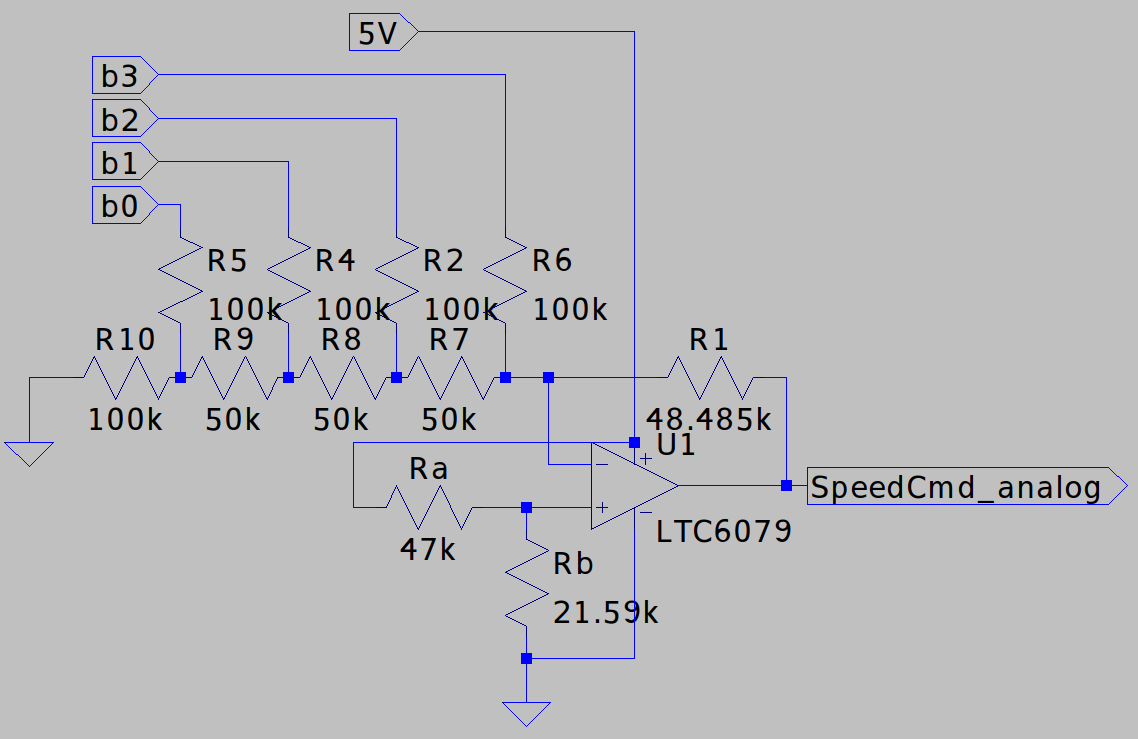
\includegraphics[width=0.42\textwidth]{dac_circuitDiagram}
  \caption{Digital to Analog Converter Circuit Diagram}
  \label{fig:dac_circuitDiagram}
\end{figure}